\documentclass[
% -- opções da classe memoir --
    12pt,       % tamanho da fonte
    %openright, % capítulos começam em página ímpar
    %twoside,   % frente e verso
    oneside,    % apenas um lado
    a4paper,    % tamanho do papel.
%
% -- opções da classe abntex2 --
    chapter=TITLE,	  	  % títulos de capítulos em letras maiúsculas
    %section=TITLE,		  % títulos de seções em letras maiúsculas
    %subsection=TITLE,	  % títulos de subseções em letras maiúsculas
    %subsubsection=TITLE, % títulos de sub-subseções em letras maiúsculas
%
% -- opções do pacote babel --
    english,			  % idioma adicional para hifenização
    % french,			  % idioma adicional para hifenização
    % spanish,            % idioma adicional para hifenização
    brazil				  % o último idioma é o principal do documento
%
]{abntex2}

\usepackage{mystyle}
\newcommand{\productname}{Automail\=/X}

% -----------------------------------------------------------------------------
% Informações de dados para CAPA e FOLHA DE ROSTO
% -----------------------------------------------------------------------------
% \title{\productname: Uma prótese robótica para geração de ações em movimentos baseada em \textcolor{red}{padrões musculares \textbf{[trocar]}}}
\title{\productname: Prótese Robótica Autônoma para a Previsão de Movimentos de Caminhada baseada em Padrões Musculares}
\titulo{\uppercase{\thetitle}}

\author{Rodrigo dos Santos Tavares}
\autor{\uppercase{\theauthor}}

\local{Boa Vista --- RR}

\date{2019}
\data{\thedate}
\orientador{Dr.\ Herbert Oliveira Rocha}

\tipotrabalho{Monografia}

\preambulo{Monografia de Graduação apresentada ao Departamento de Ciência da
  Computação da Universidade Federal de Roraima como requisito parcial para a
  obtenção do grau de Bacharel em Ciência da Computação.}

% -----------------------------------------------------------------------------


% -----------------------------------------------------------------------------
% Informações de dado para a FOLHA DE APROVAÇÃO
% -----------------------------------------------------------------------------
\renewcommand{\dataDefesa}{10 de julho de 2019}
\renewcommand{\orientadorBanca}{Prof.\ Dr.\ Herbert Oliveira Rocha}
\renewcommand{\primeiroMembroBanca}{Prof.\ Dr.\ Leandro Nelinho Balico}%TODO:Membros da banca
\renewcommand{\segundoMembroBanca}{Prof.\ Dr.\ Luciano Ferreira Silva}
% -----------------------------------------------------------------------------

% \addto\captionsportuguese{\renewcommand{\refname}{Reference}}
% \renewcommand{\refname}{Reference}
% \renewcommand{\bibsection}{REF}

% -----------------------------------------------------------------------------
% compila o índice
% -----------------------------------------------------------------------------
\makeindex
% -----------------------------------------------------------------------------

% -----------------------------------------------------------------------------
% Início do documento
% -----------------------------------------------------------------------------
\begin{document}

% Retira espaço extra obsoleto entre as frases.
%\frenchspacing

% -----------------------------------------------------------------------------
% ELEMENTOS PRÉ-TEXTUAIS
% -----------------------------------------------------------------------------
% \pretextual

% -----------------------------------------------------------------------------
% Capa
% -----------------------------------------------------------------------------
\imprimircapa{}
% -----------------------------------------------------------------------------

% -----------------------------------------------------------------------------
% Folha de rosto
% (o * indica que haverá a ficha bibliográfica)
% -----------------------------------------------------------------------------
\imprimirfolhaderosto{}
% -----------------------------------------------------------------------------

% -----------------------------------------------------------------------------
% Inserir folha de aprovação
% -----------------------------------------------------------------------------
\imprimirfolhadeaprovacao{}
% -----------------------------------------------------------------------------

% -----------------------------------------------------------------------------
% Dedicatória
% -----------------------------------------------------------------------------
% \begin{dedicatoria}
%   \vspace*{\fill}
%   \centering
%   \noindent
%   \todo{Dedicatória}\textcolor{red}{Dedico este trabalho a \lipsum[1]} \vspace*{\fill}%TODO: Dedicatória
% \end{dedicatoria}
% -----------------------------------------------------------------------------

% -----------------------------------------------------------------------------
% Agradecimentos
% -----------------------------------------------------------------------------
% \begin{agradecimentos}[Agradecimentos]
%   \todo{Agradecimentos}\textcolor{red}{\lipsum[1]}%TODO:Agradecimentos
% \end{agradecimentos}
% -----------------------------------------------------------------------------

% -----------------------------------------------------------------------------
% Epígrafe
% -----------------------------------------------------------------------------
% \begin{epigrafe}
%     \vspace*{\fill}
% 	\begin{flushright}
% 		\textit{???????????} %TODO: Epígrafe
% 	\end{flushright}
% \end{epigrafe}
% -----------------------------------------------------------------------------

% -----------------------------------------------------------------------------
% RESUMOS
% -----------------------------------------------------------------------------
\setlength{\absparsep}{18pt} % ajusta o espaçamento dos parágrafos do resumo

% -----------------------------------------------------------------------------
% PORTUGUÊS
% -----------------------------------------------------------------------------
\begin{resumo}[Resumo]
  Pessoas com membros inferiores amputados geralmente buscam próteses que os ajudem a realizar as tarefas cotidianas, porém as próteses mais comuns do mercado com preços mais acessíveis são passivas e carecem de funcionalidades que podem trazer mais naturalidade aos movimentos do usuário. Este trabalho propõe o projeto de uma prótese robótica para o pé humano que funcione de forma autônoma através da previsão de movimentos das articulações com o intuito de auxiliar na locomoção de seu usuário e monitore dados relacionados à saúde do usuário através de técnicas de aprendizado de máquina. Visando baixo custo por meio de componentes encontrados no mercado nacional e por meio de impressão da estrutura/frames com impressora 3D. Com o foco na garantia da qualidade do produto, o processo de desenvolvimento do sistema proposto será demonstrado com a aplicação de técnicas de métodos formais para validá-lo, tais como, redes de Petri e \textit{model checkers}.

 \vspace{\onelineskip}

 \noindent
 \textbf{Palavras-chave}: próteses, robótica de reabilitação, sistemas embarcados, acelerômetro, giroscópio
\end{resumo}
% -----------------------------------------------------------------------------

% -----------------------------------------------------------------------------

% -----------------------------------------------------------------------------
% INGLÊS
% -----------------------------------------------------------------------------
% \begin{resumo}[Abstract]
%  \begin{otherlanguage*}{english}
%     People with amputated lower limbs usually seek prostheses that help them perform everyday tasks, but the most common ones available with accessible prices are passive prostheses and lack features to make the user's movements more natural. This work proposes the design of a robotic prosthesis for the human foot that aids people in locomotion and tracks data relating to the user's health through machine learning techniques, targeting low cost by means of 3D printing. Part of this project is also using formal methods to validate it.
  
%   \vspace{\onelineskip}

%     \noindent
%     \textbf{Keywords}: prostheses, rehabilitation robotics, embedded systems, accelerometer, gyroscope
%  \end{otherlanguage*}
% \end{resumo}
% -----------------------------------------------------------------------------

% -----------------------------------------------------------------------------

% -----------------------------------------------------------------------------
% Lista de ilustrações
% -----------------------------------------------------------------------------
\pdfbookmark[0]{\listfigurename}{lof}
\renewcommand{\listfigurename}{Lista de Figuras}
\listoffigures*
\cleardoublepage{}
% -----------------------------------------------------------------------------

% -----------------------------------------------------------------------------
% Lista de tabelas
% -----------------------------------------------------------------------------
% \pdfbookmark[0]{\listtablename}{lot}
% \renewcommand{\listtablename}{Lista de Tabelas}
% \listoftables*
% \cleardoublepage{}
% -----------------------------------------------------------------------------

% -----------------------------------------------------------------------------
% Lista de abreviaturas e siglas
% -----------------------------------------------------------------------------
% \begin{siglas}
%   \item[FSM] Máquina de Estados Finita (\textit{Finite State Machine})
%   \item[IoT] Internet das Coisas (\textit{Internet of Things})
%   \item[SVM] Máquina de Vetor de Suporte (\textit{Support Vector Machine})
%   %TODO: Não esquecer de completar essa lista
% %    \item[EDS] Exemplo De Sigla
% \end{siglas}
% -----------------------------------------------------------------------------

% -----------------------------------------------------------------------------
% Lista de símbolos
% -----------------------------------------------------------------------------
% \begin{simbolos}
%   \item[$ \Gamma $] \todo{Atualizar esta lista!} Letra grega Gama
%   \item[$ \Lambda $] Lambda
%   \item[$ \zeta $] Letra grega minúscula zeta
%   \item[$ \in $] Pertence
% \end{simbolos}
% -----------------------------------------------------------------------------

% -----------------------------------------------------------------------------
% Sumário
% -----------------------------------------------------------------------------
\pdfbookmark[0]{\contentsname}{toc}
\renewcommand{\contentsname}{Sumário}
\tableofcontents*
\cleardoublepage{}
% -----------------------------------------------------------------------------



% -----------------------------------------------------------------------------
% ELEMENTOS TEXTUAIS
% -----------------------------------------------------------------------------
\textual{}
% -----------------------------------------------------------------------------
% Introdução
% -----------------------------------------------------------------------------
\chapter{Introdução}\label{ch:introducao}
% ----------------------------------------------------------
% INTRODUÇÃO
% ----------------------------------------------------------
Soluções tecnológicas são desenvolvidas cada vez mais para suprir necessidades que melhorem a qualidade de vida das pessoas. Quando nos tornamos incapazes de interagir fisicamente com o ambiente ao nosso redor, buscamos este tipo de solução. O campo da robótica de reabilitação visa trazer conforto e restaurar a independência de pessoas com limitações, incluindo pessoas com membros amputados, que precisam de próteses para voltar às atividades cotidianas \cite{siciliano:2008}.

Segundo \citeonline{siciliano:2008}, o desafio do desenvolvimento de próteses de membros humanos é manter a funcionalidade de um membro natural. Aspectos desta naturalidade incluem controle intuitivo das articulações, controle da força dos membros para situações diversas, e sentidos tátil e de movimento que existem nos membros naturais.

As próteses mais comuns para membros inferiores são otimizadas para caminhada em linha reta e, por isso, têm rigidez fixa nas articulações, o que dificulta várias ações do cotidiano que fogem desse comportamento padrão \cite{pew:2017}. Conforme a análise de \citeonline{dedic:2011}, próteses comerciais ainda costumam ser passivas mesmo com o avanço tecnológico dos últimos anos, e muitas funções motoras exigem uma energia maior nas articulações.

De acordo com \citeonline{novak:2013Automated}, vários dispositivos que visam aprimorar ou restaurar funções motoras de membros inferiores foram desenvolvidos, incluindo exoesqueletos e próteses ativas. Estes sistemas são equipados com sensores utilizados para perceber o ambiente ao redor do corpo humano. Além de sensores localizados nos dispositivos em si, também existem sistemas com sensores como acelerômetros montados no corpo do usuário, com o intuito de compreender as intenções do usuário e prever seus movimentos.

Para que ações como subir escadas e rampas sejam realizadas naturalmente, é necessário que se utilize mais energia nas articulações, que precisam de mais força nessas ações do que na caminhada plana. Mesmo com o controle computadorizado de articulações que permitem velocidades diferentes de caminhada, ainda é difícil para pessoas amputadas a subida de escadas \cite{dedic:2011}.

Com o advento das próteses ativas, fez-se possível definir estratégias de controle diferentes para cada tipo de ação do usuário. Isto acontece porque a biomecânica da perna é bem variável em relação à ação realizada, dependendo se o indivíduo está caminhando em um chão plano, ou subindo ou descendo uma rampa ou escada, por exemplo. Um campo de pesquisa atual consiste em determinar precisa e rapidamente o tipo de ação que o usuário está realizando, sem que seja necessário um dispositivo externo à prótese \cite{stolyarov:2017}.

Ainda segundo \citeonline{stolyarov:2017}, os métodos mais eficazes de prever estas ações de caminhada atualmente envolvem reconhecimento de padrões de sensores como unidades de medição inerciais, (IMUs) e eletrodos de eletromiografia superficial (sEMG), que é um método que varia muito fora de ambientes de laboratório, pois depende de diversos fatores fisiológicos.

\todo[inline]{concluir a introdução com a motivação}


% ----------------------------------------------------------
% PROBLEMA
% ----------------------------------------------------------
\section{Definição do Problema}
\todo[inline]{Escrever a definição do problema acima}%TODO
O problema abordado por este trabalho é representado pelo seguinte questionamento: \textit{Como projetar uma prótese robótica para a perna humana que funcione de forma autônoma através da previsão de movimentos das articulações com o intuito de auxiliar na locomoção de seu usuário, visando um baixo custo e permitindo o monitoramento da saúde de seu usuário em situações de perigo?}	

% ----------------------------------------------------------
% OBJETIVOS
% ----------------------------------------------------------
\section{Objetivos}
\label{sec:objetivos}
%\todo{Revisar, foi atualizado, pois está muito parecido com a questão de pesquisa, aqui temos que uma resposta}
O objetivo geral deste trabalho é projetar e desenvolver uma prótese robótica que seja autônoma por meio da previsão de movimentos das articulações do usuário durante as ações executadas, utilizando-se de modelos formais para validar a ações do sistema proposto e a definição de dados a serem coletados durante sua execução, bem como a utilização de sensores de movimento, pressão, motores disponíveis no mercado nacional e estruturas feitas em impressora 3D, visando o baixo custo de produção.

%O objetivo geral deste trabalho é projetar e desenvolver uma prótese robótica que seja autônoma para usuário por meio da previsão de movimentos de suas articulações durante as ações executadas, ao mesmo tempo deve ser de baixo custo e efetuar monitoramento da saúde de seu usuário.

Os objetivos específicos são os seguintes:
\begin{enumerate}
  \item Identificar métodos para a modelagem do software e do hardware;
  \item Definir um modelo formal que represente o fluxo de execução do sistema proposto, visando analisar propriedades de segurança;
  \item Demonstrar uma técnica para transformação de modelos de software em códigos do projeto;
  \item Propor um método para prever movimentos de articulações através da classificação de sinais extraídos do membro residual;
  \item Determinar componentes eletrônicos de baixo custo para a prototipação do sistema proposto;
  \item Construir uma estrutura para prótese utilizando impressora 3D.
  \item Propor uma técnica que analise os dados dos sensores e o funcionamento do sistema, afim de prever perigos à saúde do usuário relacionados ao uso da prótese como, por exemplo, postura incorreta;
  \item Validar sistema proposto pela análise de testes práticos e simulados, a fim de examinar a sua eficácia e aplicabilidade.
\end{enumerate}

% ----------------------------------------------------------
% METODOLOGIA
% ----------------------------------------------------------
\section{Metodologia Proposta}
\label{sec:metodologia}

% ----------------------------------------------------------
% CONTRIBUIÇÕES
% ----------------------------------------------------------
\section{Contribuições Propostas}
\label{sec:contribuicoes}

% ----------------------------------------------------------
% ORGANIZAÇÃO
% ----------------------------------------------------------
\section{Organização do Trabalho}
\label{sec:organizacao}


% -----------------------------------------------------------------------------
% Conceitos e Definições
% -----------------------------------------------------------------------------
\chapter{Conceitos e Definições}\label{ch:fundamentacao}
\section{Sistemas Embarcados}
\label{sec:embarcados}
Sistemas computacionais fazem parte de diversos produtos desde computadores pessoais e \textit{laptops}, até utensílios domésticos. Destes sistemas, são conhecidos como embarcados os que fazem parte de um dispositivo eletrônico maior, não representando sua totalidade, mas oferecendo recursos computacionais \cite{vahid:2002}. Entende-se por sistema embarcado um sistema computacional de propósito específico -- em contraste a um computador pessoal --, que não assume vários papéis de acordo com a necessidade do usuário, apenas realiza tarefas predeterminadas \cite{heath:2002}. Isto é, são sistemas eletrônicos projetados para funções específicas dentro de um dispositivo maior, que pode controlar o meio físico e permite sua interação com o usuário.

\todo{Fazer gancho para próxima seção}
\subsection{Microcontroladores vs. Microprocessadores}
Microcontroladores são processadores com vários componentes embutidos, como RAM, uma memória de programa e interfaces de entrada e saída \cite{white:2011}. Os microcontroladores surgiram como um substituto para circuitos lógicos discretos, por serem mais facilmente programáveis e proporcionarem uma funcionalidade maior \cite{heath:2002} e, segundo \citeonline{marwedel:2010}, grande parte dos processadores em sistemas embarcados são, na verdade, microcontroladores, por serem simples e fáceis de usar.

A distinção entre microprocessadores e microcontroladores é difícil de ser feita, \citeonline{schlett:1998} diz que, de forma simplificada, é comum diferenciá-los considerando seu desempenho, considerando dispositivos de 8 e 16-bit como microcontroladores, e a partir disto como microprocessadores.

\todo{Falta alguma coisa, talvez.}	

\subsection{IoT: Internet das Coisas}
Com a constante evolução e a ubiquidade da Internet, começam a surgir objetos conectados, transformando dispositivos que já faziam parte do cotidiano em algo que possa ser autônomo e inteligente \cite{kopetz:2011}.  Segundo \citeonline{xia:2012}, o termo ``Internet das Coisas''  não refere-se apenas à existência destes dispositivos inteligentes, mas à interconexão dos objetos do cotidiano através de sistemas embarcados, proporcionando assim ambientes em que os dispositivos se comunicam entre si e também com seres humanos.

\section{Robótica e suas Aplicações}
\label{sec:robotica}
\subsection{Próteses Robóticas}
\todo[inline]{Próteses ativas, passivas, eletromiográficas}

\section{Eletromiografia: Geração de Dados}
\label{sec:emg}
\todo[inline]{Como funciona, de onde vêm os dados, etc.}

\section{Reconhecimento de Padrões}
\label{patternrec}
Nesta seção serão abordados aspectos relevantes ao reconhecimento dos padrões dos sinais, desde seu pré-processamento a previsões dos movimentos do usuário.
\subsection{Pré-processamento}
\todo[inline]{Filtros e fusão de dados, provavelmente?}%TODO
\subsection{Aprendizado de máquina}
\todo[inline]{Dizer aqui que nas próximas seções serão abordados alguns dos principais métodos de classificação}%TODO
\subsubsection{Árvores de decisão}
\todo[inline]{SciKit-Learn usa uma versão otimizada do algoritmo CART}%TODO
\subsubsection{SVM e outros}

\todo[inline]{É necessário falar sobre impressora 3D, caso eu pretenda usar uma?}
\todo[inline]{Herbert: Não, falaremos na introdução}

\section{Modelos Formais para Validação de Sistemas}
\label{sec:modelosformais}
\subsection{Autômatos}
\subsection{Redes de Petri}

\section{Modelagem de software}
\label{sec:modelagem}
\subsection{Transformações de modelo para código}

% -----------------------------------------------------------------------------
% Revisão de Literatura
% -----------------------------------------------------------------------------
\chapter{Trabalhos Correlatos}\label{ch:correlatos}
Este capítulo apresentará outros trabalhos existentes na literatura que compartilham de objetivos semelhantes ou são comparáveis de alguma forma e contribuem para o desenvolvimento deste trabalho. Os trabalhos a seguir propõem métodos para previsão de movimentos para próteses ativas.

\section{Translational Motion Tracking of Leg Joints for Enhanced Prediction of Walking Tasks}
\cite{stolyarov:2017}

\section{Turn Intent Detection for Control of a Lower Limb Prosthesis}
\cite{pew:2017}

\section{Automated detection of gait initiation and termination using wearable sensors}
\cite{novak:2013Automated}

\section{A Novel Design of a Full Length Prosthetic Robotic Arm for the Disabled}
\cite{kumar:2017}

\section{SmartLeg: An intelligent active robotic prosthesis for lower-limb amputees}
Foi proposto por \citeonline{dedic:2011} uma forma de transformar uma prótese passiva disponível comercialmente em ativa, para que seja possível a subida e descida de escadas e outros movimentos que exigem energia externa. Como para subir escadas é importante a presença do joelho e de mais força, faz-se necessário o uso de uma fonte de energia externa, que foi feita usando atuadores hidráulicos nas articulações. \citeonline{dedic:2011} também discutem o uso de aprendizagem de máquina para garantir conforto aos usuários, pois pode-se adaptar os atuadores para funcionarem melhor com os padrões de andadura da pessoa, mas isso não foi implementado.

\section{Evaluation of shoulder complex motion-based input strategies for endpoint prosthetic-limb control using dual-task paradigm}
\cite{losier:2011}

\section{Movement error rate for evaluation of machine learning methods for sEMG-based hand movement classification}
\cite{gijsberts:2014}



% -----------------------------------------------------------------------------
% Detalhes de Desenvolvimento do Projeto
% -----------------------------------------------------------------------------
\chapter{Método Proposto}\label{ch:metodo}
Este capítulo apresentará o método proposto por este trabalho para o projeto de prótese ativa baseada em sensores e aprendizado de máquina.

\section{\todo{Corrigir este título}A prótese}
\label{sec:metodo_protese}
\todo[inline]{Explicar o funcionamento geral, relacionando à big picture}
\label{sec:metodo_geral}
\begin{figure}[h]
	\caption{\label{fig:big_picture}Visão geral do protótipo}
	\begin{center}
	    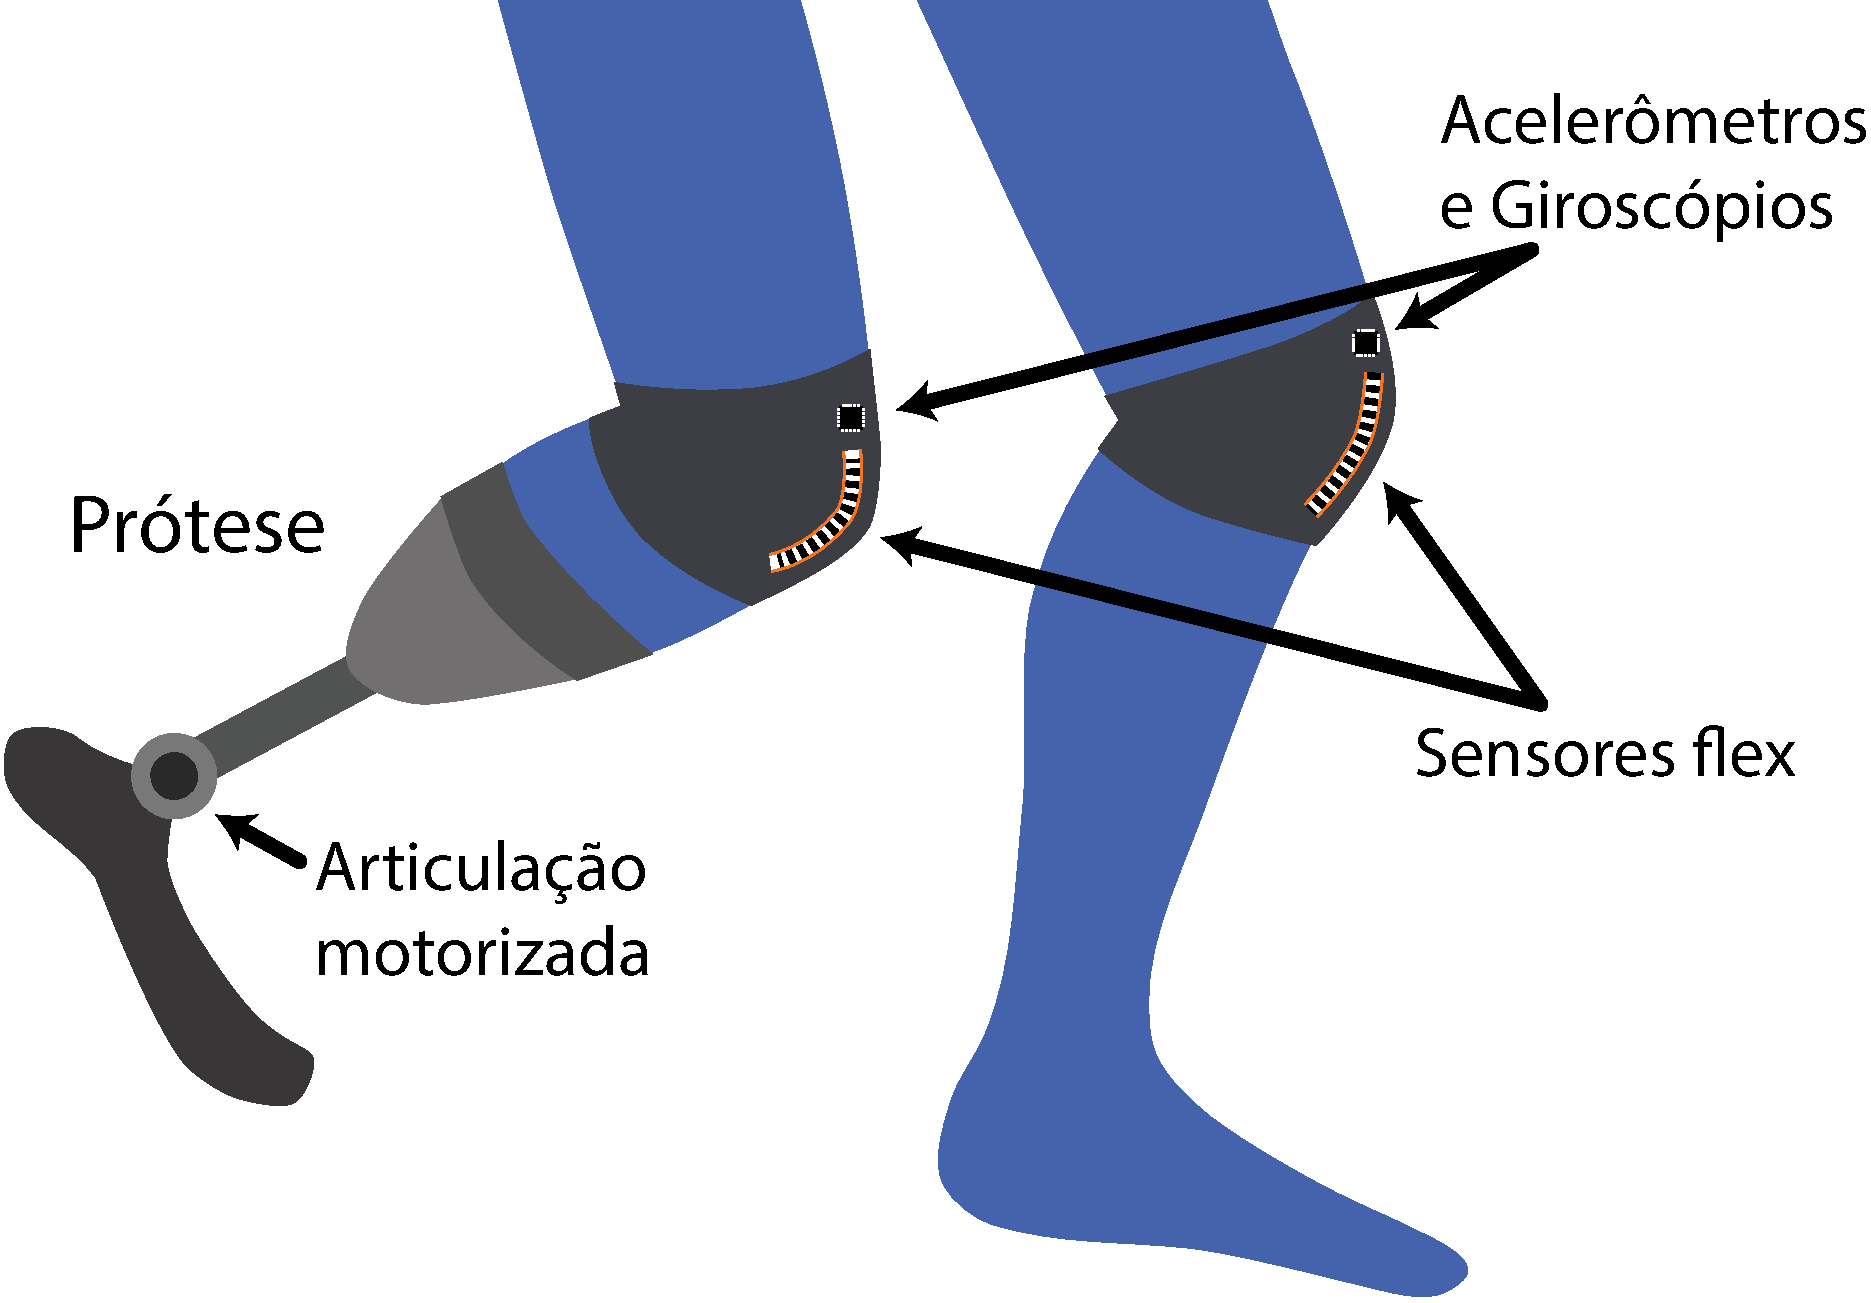
\includegraphics[width=0.8\textwidth]{resources/big_picture}
	\end{center}
	\legend{Fonte: Elaborada pelo autor}
\end{figure}

\todo[inline,color=lightgray]{Projeto e prototipação de uma prótese robótica para pé\\Como criar;\\Onde vão estar os sensores, materiais de baixo custo, próteses 3D;\\O que a prótese gera?; Atuadores; Gerar perguntas.}
\todo[inline]{Como vai ser a fonte de energia da prótese?}

\section{Coleta de dados e classificação}
\todo[inline,color=lightgray]{Coleta de dados dos sensores -- que sensores, que dados. Por que os dados são importantes: usar técnicas pra prever e identificar dados (Seção explicando da coleta, uma seção pra cada tipo de classificação)}

\todo[inline]{\textbf{Nova seção?}}
\todo[inline,color=lightgray]{Geração de movimentos: a partir dos dados coletados. Os atuadores vão tentar identificar os ambientes. Na escada, o motor vai fazer tal coisa, etc. Na rampa, etc.}

\todo[inline]{\textbf{Nova seção?}}
\todo[inline,color=lightgray]{Analisar saúde do caminhar. Se não tá caminhando torto. Gerar estatísticas do uso da prótese. (Os dados estão fazendo a pessoa puxar mais pra uma perna)}


% -----------------------------------------------------------------------------
% Resultados Experimentais
% -----------------------------------------------------------------------------
\chapter{Avaliação Experimental}\label{ch:resultados}
Este capítulo aborda a execução do método proposto por este trabalho e a análise dos resultados obtidos pelos experimentos realizados a fim de verificar a viabilidade do projeto, bem como sua eficiência.

\section{Planejamento}\label{sec:result_planejamento}
O intuito desta avaliação experimental é verificar a capacidade do sistema AutomailX de exibir um objeto 3D animado e classificar as ações do usuário a partir da leitura dos sensores do protótipo.

\todo{\textbf{Coesão:} ``Para este fim...''} Utilizou-se um Arduino Uno, um sensor MPU-6050 e um sensor flexível\todo{especificar sensores} para a captura dos dados de movimento do usuário. Todos estes equipamentos foram fixados \todo{qual o nome da luvinha de joelho} no joelho direito dos sujeitos de teste, simulando a pena que estaria utilizando a prótese.

Foram selecionados indivíduos para gerar o conjunto de dados que seria utilizado para a classificação, e solicitado para que cada um deles caminhasse em linha reta, enquanto era capturado o estado da transição de cada uma das ações. A captura foi feita a partir de um cabo USB conectado a um notebook \todo{configuração} estabelecendo conexão via porta serial para o programa.

As ações definidas para este experimento foram apenas voltadas à detecção de uma caminhada plana, classificando cada um dos passos de cada perna\todo{devido à limitação dos sensores disponíveis, pois o giroscópio não é tão preciso assim sozinho}{ }.

A simulação animada em 3D mostra em tempo real o movimento realizado pelos dois sensores e, após a captura dos dados, mostra também a ação realizada na prótese simulada, baseado na classificação dos dados de movimento.

\section{Execução da avaliação experimental}\label{sec:result_execucao}
\todo[inline]{Dado tal cenário, coletei os dados, funcionou mas poderia melhorar de tal jeito, isso e aquilo. Se não funcionou, pode ter sido limitação do classificador, ou do sensor, ou da placa.}
\todo[inline]{Escolha do algoritmo, comparação de gráficos
}

% -----------------------------------------------------------------------------
% Considerações Finais e Trabalhos Futuros
% -----------------------------------------------------------------------------
\chapter{Conclusões e Trabalhos Futuros}\label{ch:consideracoes}
Este trabalho abordou o desenvolvimento de uma prótese robótica para o pé humano com o intuito de melhorar a qualidade de vida de pessoas com amputações, através do uso de aprendizado de máquina.

No decorrer do trabalho, foi possível observar várias abordagens a problemas semelhantes, que servirão de base para tomar certas decisões como o algoritmo de aprendizado de máquina a ser utilizado.

Foi planejado o funcionamento da prótese, incluindo o fluxo de funcionamento do \textit{software}, contendo a classificação e previsão de movimentos do usuário. Neste contexto, foi elaborado um diagrama de sequência.

No futuro, planeja-se elaborar uma rede de Petri a partir do diagrama de sequência, para que possa ser validada antes que o \textit{software} seja desenvolvido. Em seguida, será construído o \textit{software} e confeccionada a prótese e todo o sistema de sensores e atuadores. Assim, será possível fazer o treinamento do modelo de aprendizado de máquina.

Também deverão ser investigadas formas de analisar a saúde do usuário de acordo com diretrizes ortopédicas, para que sejam usadas usadas em um relatório gerado a partir dos dados dos sensores.

% -----------------------------------------------------------------------------
% Cronograma
% -----------------------------------------------------------------------------
% \chapter{Cronograma}\label{ch:cronograma}
% A \autoref{tab:cronograma} exibe o cronograma proposto para a próxima etapa do trabalho de conclusão de curso, essas atividades são:

\begin{table}[htbp]
  \centering
  \caption{Cronograma de atividades}
  \label{tab:cronograma}
  \begin{tabularx}{\textwidth}{|X|c|c|c|c|c|}
    \hline
    \textbf{Atividade} & \textbf{Agosto} & \textbf{Setembro} & \textbf{Outubro} & \textbf{Novembro} & \textbf{Dezembro} \\
    \hline
    Criação de modelo formal & \(\times\) & & & & \\
    \hline
    Validação de modelo & \(\times\) & \(\times\)  &  & & \\
    \hline
    Desenvolvimento de software de classificação & & \(\times\) & \(\times\) & \(\times\) & \\
    \hline
    Confecção da prótese e aparato de sensores & \(\times\) & \(\times\) & & &  \\
    \hline
    Treinamento do modelo de aprendizado de máquina & & & \(\times\) & &  \\
    \hline
    Testes com o protótipo da prótese & & & \(\times\) & \(\times\) &  \\
    \hline
    Escrita do TCC & & & \(\times\) & \(\times\) &  \(\times\)\\
    \hline
    Defesa para a banca & & & & & \(\times\)  \\
    \hline
  \end{tabularx}
  %\legend{Fonte: Autor.}
\end{table}

%\newpage
% -----------------------------------------------------------------------------
% Referências bibliográficas
% -----------------------------------------------------------------------------
%\bibliographystyle{abnt-alf}
\renewcommand{\bibname}{Referências}
\bibliography{main}


% -----------------------------------------------------------------------------
% ÍNDICE REMISSIVO
% -----------------------------------------------------------------------------
%\phantompart
\printindex
% -----------------------------------------------------------------------------

\end{document}
